\documentclass[main.tex]{subfiles}
\begin{document}

\chapter{Results}\label{ch:results}

\section{Data Sets}
\subsection{Overview and Comparison}
The data presented here were collected during a one-hour measurement with both the analog and the digital setup running in parallel. A total of 4.3 million pulses from the NE213 detector were recorded by the analog setup. The digitizer saw 2.2 million pulses from the NE213 detector over the same period of time. This large difference in counts was because the digital setup was configured to transfer each event individually, resulting in a very low livetime.
In the analog setup, amplitude thresholds of 25.0 mV and 94.6 mV were applied to the YAP detector and the NE213 detector, respectively. In the digital setup, thresholds of 9.8 mV and 48.8 mV were applied to the YAP detector and the NE213 detector, respectively. Having such a low threshold on the YAP detector was found to decrease the signal-to-noise ratio in the ToF spectrum, so a higher threshold of \SI{24.4}{\milli\volt} was applied offline in software. Table \ref{tab:settings} presents an overview of the data sets.
\begin{table}[bh]
\center
\begin{tabular}{|l|l|l|l|l|}
\hline 
Setup   & \shortstack{YAP \\threshold (mV)}  & \shortstack{NE213 \\ threshold (mV)} & \shortstack{NE213 \\ events ($\text{10}^\text{6}$)} & \shortstack{Livetime\\ \%} \\ \hhline{|=|=|=|=|=|}
Analog  & 25.0              & 94.6                & 4.3      & 44             \\ \hline
Digital & 9.8/24.4*			& 48.8                & 2.2      & **             \\ \hline
\end{tabular}
\caption[Overview of the analog and digital data sets.]{Overview of the analog and digital data sets. *An amplitude threshold of \SI{24.4}{mV} was enforced offline (see text for details). **The digital setup did not have a method for determining livetime.}
\label{tab:settings}
\end{table}



\subsection{Livetime and Threshold Alignment}
\subsubsection{Deposited Energy}
The analog and the digital setups were run with different amplitude thresholds. To properly compare them, a common threshold was necessary. Further, the analog and digital setups had significantly different cable lengths between the detectors and the electronics. Thus, the signals were attenuated differently before being processed by the different systems. As a result, the required digital-setup threshold was significantly higher than the analog threshold.

\begin{figure}[h!]
    \centering
        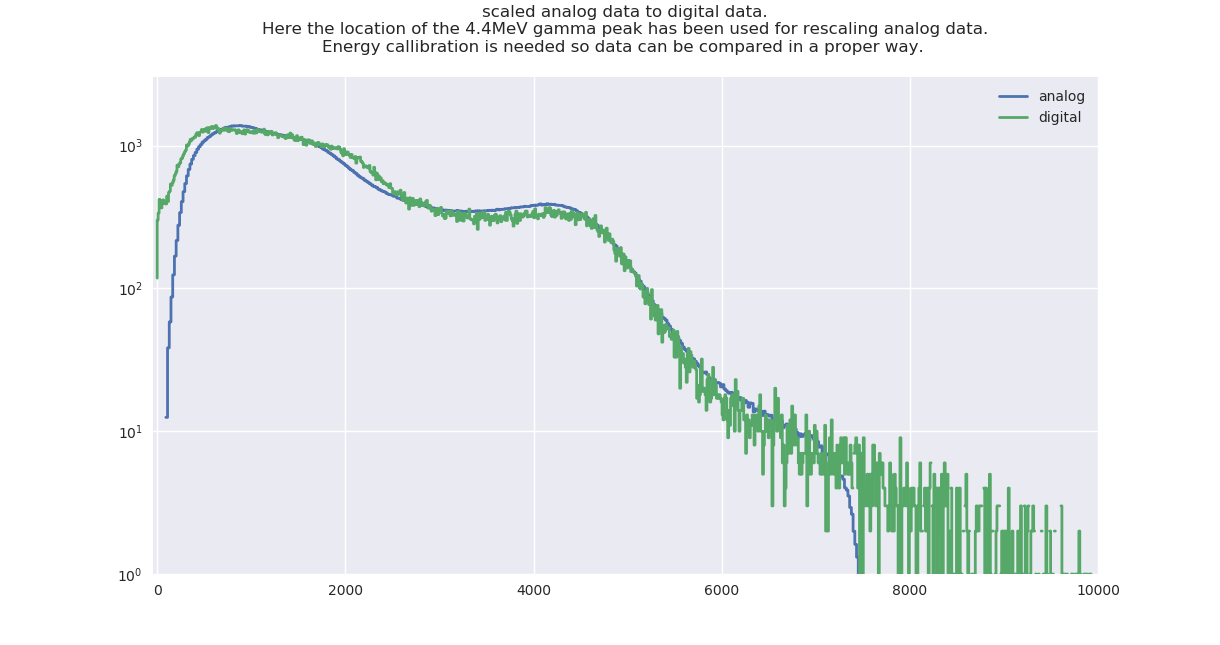
\includegraphics[width=0.7\textwidth]{CompareResults/qdc_comp.pdf}
        \caption[Comparison of analog and digital spectra from the NE213 detector.]{Comparison of analog and digital spectra from the NE213 detector. Top: Livetime-corrected analog energy spectrum (red). Raw digital energy spectrum (blue). Digital energy spectrum after threshold matching and normalization (green). Bottom: Ratio of counts between the livetime-corrected analog spectrum and the normalized digital spectrum.}
    \label{fig:qdc_comp}
\end{figure}
Figure~\ref{fig:qdc_comp} (top panel) shows the energy spectra from both setups. The data from the analog setup have been livetime corrected (44\%). The blue histogram shows the raw digital spectrum, and the green histogram shows the digital spectrum after applying a higher amplitude threshold of \SI{151}{mV} in software and normalizing the spectrum to match the height of the livetime-corrected analog setup. The resulting red and green spectra are far more similar, although the Compton edges associated with the \SI{4.44}{\MeV}$_\textrm{ee}$ gamma-ray do not look exactly the same. This may be because some of these gamma-rays deposited energies which exceeded the dynamic range of the digitizer. 
The livetime of the digital setup can be estimated by scaling the livetime of the analog setup to the ratio of counts in the digital and analog setups. A crude estimate of the livetime of the digital setups is thus 22\%.
Figure~\ref{fig:qdc_comp} (bottom panel) shows the ratio between the digital and analog spectra as a function of deposited energy after both threshold alignment and normalization. Ideally, this ratio should be unity. This is not the case. Near the Compton edge corresponding to the \SI{4.44}{\MeV}$_\textrm{ee}$ gamma-ray there is a bump and a valley. Again, this may be due to the highest amplitude digitized pulses corresponding to the highest energy Compton scattering events being clipped, causing them to register lower values of deposited energy.


\subsubsection{Time-of-Flight Spectra}
The ToF spectrum is heavily influenced by the choice of amplitude threshold. Figure~\ref{fig:tof_comp} (top panel) shows ToF spectra for the two setups with the initial 49 mV NE213 detector threshold on data from the digital setup and a 94.6 mV threshold on the data from the analog setup. Interestingly, it seems that the analog setup misses the less energetic neutrons due to the high amplitude threshold. By applying the offline NE213 detector amplitude threshold of \SI{151}{mV} and the YAP detector threshold of \SI{44}{mV} to the data from the digital setup and normalizing the data as before, the ToF spectra shown in the bottom panel of Fig.~\ref{fig:tof_comp} are obtained. The neutron peaks now have roughly the same shape, which means that the amplitude cut has also removed these lower energy neutrons.

\begin{figure}[h]
    \centering
        \includegraphics[width=0.7\textwidth]{CompareResults/tof_comp.pdf}
        \caption[Analog and digital ToF spectra.]{Analog and digital ToF spectra. Top: Unadjusted. Bottom: livetime has been taken into account and a higher threshold has been enforced on the NE213 and YAP signals for the digital setup.}
    \label{fig:tof_comp}
\end{figure}

\section{Analog Setup}

\subsection{Neutron Tagging}
Figure~\ref{fig:tof_a} shows the ToF spectrum recorded by the analog setup. The neutron and gamma-ray peaks are indicated. In addition to these two peaks, there is an approximately flat background. This background represents uncorrelated particles triggering the TDC start and stop, which is also why negative ToF values appear.
The gamma-flash has been shifted to be centered at \SI{3.8}{ns}, the time it takes light to travel from the source to the detector. The width of the gamma-flash is primarily due to the time resolution of the detectors. This depends on where in the detector volume the gamma-ray interacts. Secondary effects include signal attenuation in the cables, which might affect PS and thus rise time. This may in turn make the CFD less effective and may cause loss in the time resolution. Furthermore, the final  digitization by the TDCs may cause some loss of resolution. Differences in flight path between gamma-rays hitting the center of the NE213 detector and those that hit near the edge will be less than \SI{1}{cm}, so this will not give rise to a substantial time spread. 
\begin{figure}[ht]
    \centering
        \includegraphics[width=0.9\textwidth]{AnalogResults/tof.pdf}
        \caption[ToF spectrum, analog setup.]{ToF spectrum, analog setup. The x-axis denotes the ToF from source to NE213 detector. The neutron and gamma-ray peaks are indicated with arrows. The coincidences highlighted in red have been converted to neutron kinetic energies and are shown in the upper right insert.}
    \label{fig:tof_a}
\end{figure}
The neutron bump has more energetic neutrons at lower ToF values and less energetic neutrons at higher ToF values. Since the distance from the source to the detector is known, it is possible to convert the neutron ToF into neutron kinetic energy. A range of $1.5\--$7~\si{\MeV} was chosen. This corresponds to a time interval of $31\--$\SI{68}{\ns}. The coincidences falling in this time interval have been highlighted in red in Fig.~\ref{fig:tof_a} and the corresponding energies are shown in the insert. The spectrum obtained by Scherzinger~\cite{ScherzingerPhd} (recall Fig.~\ref{fig:scherzinger}) has been superimposed. This spectrum has been normalized to produce the best qualitative agreement possible. The Scherzinger spectrum was measured with the same source but a different and smaller NE213 detector. That detector had only $\sim$10\% of the scintillation volume of the one used here and was cylindrical. 
Low-energy neutrons are clearly missing from the current data set, likely because a too large amplitude threshold has been applied. 
It also appears that the neutron-energy spectrum acquired by the analog setup is shifted to the right by roughly half an MeV. Below \SI{2.5}{MeV}, the count rate in Fig.~\ref{fig:tof_a} increases. This is simply an effect of the last $\sim$\SI{20}{\ns} primarily consisting of background.



\subsection{Pulse-Shape Discrimination}
Neutrons and gamma-rays were discriminated using the PS parameter given in Eq.~\ref{eq:ps}. The parameters $a$=120 QDC channels and $b$=0 QDC channels were found to linearize PS as a function of energy when gate lengths of \SI{500}{\ns} and \SI{60}{ns} were used for the LG and SG integrations respectively.
PS is shown as a function of deposited energy in Fig.~\ref{fig:psd_a}. Pulses in the upper band (labeled neutrons) have a large amount of charge in the tail of the scintillation pulse. Pulses in the lower band (labeled gamma-rays) have a smaller amount charge in the tail of the scintillation pulse. 
This is confirmed by the presence of the Compton edges corresponding to \SI{2.23}{MeV} and \SI{4.44}{MeV} gamma-rays in the lower band. The amplitude threshold of \SI{94.6}{mV} gives rise to the sloping energy threshold highlighted with a red line in the figure. This is because pulses with higher PS  have more charge in the tail, so given two pulses of equal amplitude, the one with larger PS will carry more charge.
\begin{figure}[ht]
    \centering
        \includegraphics[width=\textwidth]{AnalogResults/psd_a.pdf}
        \caption[Analog PS spectrum as a function of deposited energy.]{Analog PS spectrum as a function of deposited energy. The dashed white line indicates the PSD cut. Structures due to the \SI{2.23}{MeV} and \SI{4.44}{MeV} gamma-rays are indicated. The red line indicates the amplitude threshold.}
        \label{fig:psd_a}
\end{figure}

The optimal PS-cut value of 0.259 was found by plotting a PS histogram and fitting Gaussian functions to the neutron and gamma-ray distributions, see Fig.~\ref{fig:fom_a}. The quality of separation between the two distributions may be expressed as a Figure of Merit, FoM, defined in terms of the centers, $C$, of the Gaussian functions and their full width at half maximum, $W$: 
\begin{equation}
\textrm{FoM} = \frac{C_n - C_\gamma}{W_n + W_\gamma}
\end{equation}
Figure~\ref{fig:fom_a} shows histograms of the PS parameter along with the Gaussian fits used to calculate the FoM. The corresponding parameters are listed in Table \ref{tab:fom_a}. The resulting integrated FoM was 0.58, but was found to be highly energy-threshold dependent. 

The neutron and gamma-ray distributions overlap at low deposited energies. Consequently, the PSD cut can result in misclassification. Orthogonal ToF information on particle species can be used to quantify the extent of this misclassification.
Figure~\ref{fig:tof_ps_a} shows PS plotted as a function of ToF, with neutron and gamma-ray distributions highlighted. 
These distributions are not cleanly separated by the applied PSD cut. A significant amount of both neutrons and gamma-rays are mislabeled. Often the start and stop signal will be due to uncorrelated particles, rather than the previously discussed $n\gamma$ and $\gamma\gamma$ pairs. These events are expected to form a flat background in the ToF spectrum due to low rates. This may be seen in Fig. \ref{fig:tof_a} at times longer than \SI{50}{ns}. Since the events still represent either neutrons or gamma-rays (ignoring the occasional muon), one would expect them to be clearly separated into two bands in Fig.~\ref{fig:tof_ps_a}. This is not the case.


\begin{figure}[h!]
	    \centering
    	    \includegraphics[width=0.9\textwidth]{CompareResults/FOM_analog.pdf}
    \caption[PS FoM for the analog setup.]{PS FoM for the analog setup.}
    \label{fig:fom_a} 
\end{figure}
\begin{table}[h]
\center
\begin{tabular}{|l|l|l|l|l|l|}
\hline
FoM  & Cut   & $W_\gamma$ & $C_\gamma$ & $W_\textrm{n}$ & $C_\textrm{n}$ \\ \hhline{|=|=|=|=|=|=|}
0.58 & 0.259 & 0.07          & 0.204           & 0.09              & 0.301               \\ \hline
\end{tabular}
\caption{CC FoM parameters for the analog setup.}
\label{tab:fom_a}
\end{table}




\begin{figure}[h!]
    \centering
        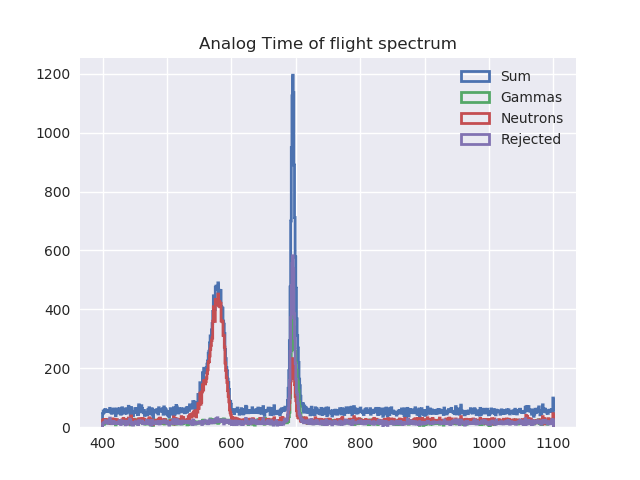
\includegraphics[width=\textwidth]{AnalogResults/tof_psd.pdf}
        \caption[PS vs. ToF for the analog setup.]{PS vs. ToF for the analog setup. The dashed white line indicates the PSD cut. Note the logarithmic z-axis.}
    \label{fig:tof_ps_a} 
\end{figure}







\newpage
\section{Digital Setup}
\subsection{Neutron Tagging}
Fig.~\ref{fig:tof_d} shows the ToF spectrum acquired with the digital setup. No additional threshold cuts or normalizations have been applied. Gamma-ray and neutron peaks are indicated. Random coincidences form a flat background. The width of the gamma-flash is again due to the intrinsic time resolution of the detectors. A secondary effect may be the digitization of the pulse. Limited resolution and sampling rate might cause the CFD algorithm to trigger slightly too soon or too late. 
The red-shaded flight times in the neutron peak have been used to generate the energy spectrum shown in the insert of Fig.~\ref{fig:tof_d}. The same time (31$\--$\SI{68}{\ns}) and energy (1.5$\--$\SI{7}{\MeV}) ranges used for the analog setup have been used here. The spectrum has far more events at lower energies than the corresponding spectrum for the analog setup, recall Fig.~\ref{fig:tof_a}. This is because the digital setup had a lower amplitude threshold than the analog setup. Thus, neutrons with less energy, which generally produce current pulses of lower amplitude in the detector, may be recorded by the digital setup. The energy spectrum looks qualitatively very similar to the superimposed reference spectrum of Scherzinger. However, the low-energy peak is located at slightly higher energy. Scherzinger might have applied an even lower threshold. 
\begin{figure}[ht]
    \centering
        \includegraphics[width=\textwidth]{DigitalResults/tof.pdf}
        \caption[ToF spectrum, digital setup.]{ToF spectrum, digital setup. The x-axis denotes the ToF from source to NE213 detector. The neutron and gamma-ray peaks have been indicated with arrows. The coincidences highlighted in red have been converted to neutron kinetic energies and are shown in the upper right insert.}
        \label{fig:tof_d} 
\end{figure}
\subsection{Pulse-shape Discrimination}
As with the analog setup, \SI{500}{ns} and \SI{60}{ns} LG and SG integration windows were used to perform PSD.  To linearize the bands, the parameters $a$ and $b$ from Eq.~\ref{eq:ps} were chosen as $a$=287 and $b$=120 (in uncalibrated digital-integration channels).
The resulting PSD spectrum is shown in Fig.~\ref{fig:psd_d}. The Compton edges corresponding to \SI{2.23}{\MeV} and \SI{4.44}{MeV} gamma-rays are indicated with arrows. A large number of low-energy gamma-rays appear at the bottom left hand corner of the plot due to the lower threshold.
A cut at PS=0.222 separates the neutron and gamma-ray bands. Again, the two distributions overlap at lower deposited energies.

\begin{figure}
    \centering
    \begin{subfigure}[ht]{\textwidth}
    	\centering
        \includegraphics[width=\textwidth]{DigitalResults/psd_d.pdf}
        \caption{}
        \label{fig:psd_d}
    \end{subfigure}
	\begin{subfigure}[ht]{\textwidth}
		\centering
        \includegraphics[width=\textwidth]{DigitalResults/CNNpsd.pdf}
        \caption{}
    	\label{fig:cnn_E} 
    \end{subfigure}
        \caption[Digital PS discrimination as a function of deposited energy.]{Digital PS discrimination as a function of deposited energy. The dashed white lines indicate PSD cuts. Structures due to the \SI{2.23}{MeV} and \SI{4.44}{MeV} gamma-rays are indicated. Top panel: CC method. Amplitude threshold is indicated with a red line. Bottom panel: CNN method.}
    \label{fig:ccm_cnn}
\end{figure}

%\subsection{Convolutional Neural Network}
The CNN described in Sec.~\ref{sec:cnn} was also applied to the digitized waveforms. The network was trained to assign a value $y$ between 0 (gamma-ray) and 1 (neutron) to each signal. The result is shown in Fig.~\ref{fig:cnn_E} as a function of deposited energy. As for the CC method, the upper distribution corresponds to neutrons and the lower distribution to gamma-rays. The two bands are separated by a PSD cut at 0.5. To highlight that the distributions overlap slightly at lower energies, the z-axis has been strongly suppressed. The CNN, trained on events from the two ToF peaks, allows for much cleaner separation between particle species, so that the exact location of the PSD cut is much less critical than in either of the CC implementations.

As for the analog setup, a FoM was calculated based on Gaussian fits to the PS distribution, see Fig. \ref{fig:fom_d}. The FoM parameters are summarized in Table \ref{tab:fom_d}. With an integrated FoM of 0.78, the digital implementation of the CC method provides better results than the analog implementation.

\begin{table}[h]
\center
\begin{tabular}{|l|l|l|l|l|l|}
\hline
FoM  & Cut   & $W_\gamma$ & $C_\gamma$ & $W_\textrm{n}$ & $C_\textrm{n}$ \\ \hhline{|=|=|=|=|=|=|}
\hline
0.78 & 0.222 & 0.07          & 0.160           & 0.11              & 0.300               \\ \hline
\end{tabular}
\caption{CC FoM parameters for the digital setup.}
\label{tab:fom_d}
\end{table}

\begin{figure}[h!]
	    \centering
    	    \includegraphics[width=0.9\textwidth]{CompareResults/FOM_digital.pdf}
	    \caption[PS FoM for the digital setup.]{PS FoM for the digital setup.}
   	    \label{fig:fom_d} 
\end{figure}

In Fig.~\ref{fig:tof_cc_tof_cnn}, the digital CC and CNN predictions are shown as functions of ToF. Figure~\ref{fig:tof_digi_cc} shows the narrow gamma-ray distribution and the wider neutron distribution as separated by the digital CC method. 
The neutron and gamma-ray background forms two slightly separated bands near prediction values 0.3 and 0.15 respectively. The two distributions overlap somewhat.  
In Fig.~\ref{fig:tof_digi_cnn}, it can be seen that the CNN method provides a much better separation, although gamma-ray and neutron distributions still overlap slightly near prediction value 0.5. The distribution of random coincidences separates into a gamma-ray band near prediction value 0 and a neutron band near 1.


\begin{figure}
    \centering
    \begin{subfigure}[ht]{\textwidth}
    	\centering
        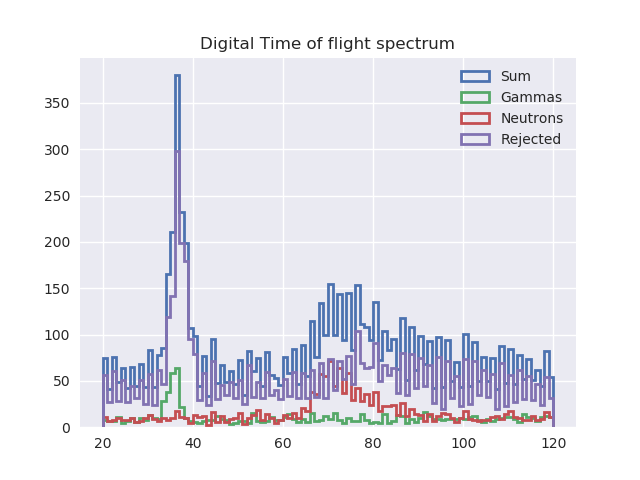
\includegraphics[width=\textwidth]{DigitalResults/tof_psd.pdf}
        \caption{}
        \label{fig:tof_digi_cc}
    \end{subfigure}
	\begin{subfigure}[ht]{\textwidth}
		\centering
        \includegraphics[width=\textwidth]{DigitalResults/CNNtof_psd.pdf}
        \caption{}
        \label{fig:tof_digi_cnn}
    \end{subfigure}
    \caption[PS vs. ToF for the digital setup.]{PS vs. ToF for the digital setup. The dashed white line indicates the PSD cut. Note the logarithmic z-axis. Top panel: CC method. Bottom panel: CNN method.}
    \label{fig:tof_cc_tof_cnn}
\end{figure}


\clearpage
\section{Misclassification}\label{sec:comp}


Another way to compare the performance of the PSD methods is by estimating the misclassification. This can be done by evaluating the ToF spectrum in three different regions and comparing the relative number of neutron and gamma-ray labeled events. It is anticipated that the number of gamma-rays identified in a background region containing only random coincidences should be the same as the number of gamma-rays identified in a chosen neighborhood of the neutron time-of-flight peak after scaling to the widths of the regions. Likewise, the number of neutrons identified at the gamma-flash should correspond to the neutron-background expectation. The misclassification of gamma-rays and neutrons, $M_{\gamma}$ and $M_{n}$ respectively, can then be expressed as

\begin{equation}
	M_\gamma(R_\gamma) = \frac{N_{n}(R_\gamma)-\langle N_n(R_\gamma)\rangle}{N_{\textrm{total}}(R_\gamma)-\langle N_n(R_\gamma)\rangle}
\end{equation}

\begin{equation}
	M_n(R_n) = \frac{N_{\gamma}(R_n)-\langle N_\gamma(R_n)\rangle}{N_{\textrm{total}}(R_n)-\langle N_\gamma(R_n)\rangle},
\end{equation}
where $N_n$ and $N_\gamma$ are the number of neutrons and gamma-rays identified in region $R$ and $N_{\textrm{total}}$ is the sum of $N_n$ and $N_\gamma$. $\langle N_n\rangle$ and $\langle N_\gamma\rangle$ are the expected numbers of neutrons and gamma-rays found by scaling the background rates to the width of $R$.
This definition of misclassification relies on the assumption that the choice of limits for each of the three regions does not seriously impact the results. The neutron peak neighborhood was set to match the range of neutron energies $1.5\--$\SI{7}{\MeV} corresponding to $31\--$\SI{68}{ns} and the gamma-flash neighborhood was selected as \SI{5}{\ns} on either side of the gamma-flash center.
It was found that as long as the peaks were contained in these regions the misclassifications changed by at most $\pm$0.5\% for the digital setup and at most $\pm$1\% for the analog setup. 


\begin{figure}
    \centering
    \begin{subfigure}[bh]{\textwidth}
   	   	\centering
	    \includegraphics[width=0.85\textwidth]{AnalogResults/ToF_filt.pdf}
    	\caption{PSD cut at PS = 0.259.}
    	\label{fig:ToF_filt_A}
   	\end{subfigure}
    \begin{subfigure}[bh]{\textwidth}
   	    \centering
        \includegraphics[width=0.85\textwidth]{DigitalResults/ToF_filt.pdf}
        \caption{PSD cut at PS=0.222.}
        \label{fig:ToF_filt_D}
    \end{subfigure}
	\begin{subfigure}[bh]{\textwidth}
	    \centering
        \includegraphics[width=0.85\textwidth]{DigitalResults/CNNToF_filt.pdf}
        \caption{PSD cut at prediction = 0.5.}
        \label{fig:ToF_filt_D_CNN}
    \end{subfigure}
	\caption[Filtered ToF spectra for misclassification studies.]{Filtered ToF spectra for misclassification studies.}
    \label{fig:tof_cc_cnn}
\end{figure}

Figure~\ref{fig:tof_cc_cnn} shows the ToF spectrum obtained with the analog setup filtered according to the CC method, as well as the ToF spectrum obtained from the digital setup filtered according to the CC and CNN methods.
For each PSD implementation, gamma-ray labeled events are blue, neutron labeled events are red and their intersection purple. 
Ideally, the intersection of the distributions should be flat. However, if there is some systematic misclassification, then the intersection will rise above the flat background level in the ToF spectrum. This may be used to quantify the misclassification of a given PSD implementation.
For the analog setup, a high degree of contamination is evident in the form of the two purple bumps coinciding with the neutron and gamma-ray peaks. This gives an estimated misclassification of 16\% for neutrons and 12\% for gamma-rays. 
The digital setup provides less misclassification with the CC method, at 12\% for neutrons and 3\% for gamma-rays. The much higher misclassification for neutrons implies that the method is biased towards gamma-rays.
The CNN approach reaches the best results with a gamma-ray misclassification of 4\% and a neutron misclassification of 5\%.
With a misclassification of nearly the same amount for both neutrons and gamma-rays, the CNN method does not appear to have a strong bias towards either particle species.
The neutron background is found to be nearly the same by the analog and digital CC methods, at 37\% and 38\% respectively. The CNN method finds a significantly higher background of neutron events at 45\%. This together with the high misclassification rates for the CC methods hints at them being biased towards gamma-rays.
The results from all three PSD implementations are summarized in Table \ref{tab:misclas}.

\begin{table}[h]
\center
\begin{tabular}{|l|l|l|l|}
\hline
& \begin{tabular}[c]{@{}l@{}}$\gamma n$-region\\ (\% misclassified)\end{tabular} & \begin{tabular}[c]{@{}l@{}}$\gamma\gamma$-region\\ (\% misclassified)\end{tabular} & \begin{tabular}[c]{@{}l@{}}Background region\\ (\% neutrons)\end{tabular} \\ \hhline{|=|=|=|=|}
\begin{tabular}[c]{@{}l@{}}CC\\ Analog\end{tabular}   & 16                                                                             & 12                                                                                 & 37                                                                        \\ \hline
\begin{tabular}[c]{@{}l@{}}CC\\ Digital\end{tabular}  & 12                                                                             & 3                                                                                  & 38                                                                        \\ \hline
\begin{tabular}[c]{@{}l@{}}CNN\\ Digital\end{tabular} & 5                                                                              & 4                                                                                  & 45                                                                        \\ \hline
\end{tabular}
\caption{Overview of PSD misclassification studies.}
\label{tab:misclas}
\end{table}

\section{Neutron Kinetic Energy and Energy Deposition}

Figure~\ref{fig:tof_E_d} shows energy deposition in the NE213 detector as a function of ToF measured with the digital setup. 
The least energetic neutrons (ToF $\sim$\SI{60}{ns}) have a smaller spread in deposited energy, whereas the faster neutrons (ToF $\sim$\SI{35}{ns}) have a much larger spread. 
This may be explained by the fact that in the NE213 detector, the neutron scatters primarily from $^1$H nuclei. Thus, by Eq.~\ref{eq:scat}, the neutron may deposit up to its entire kinetic energy in a single scatter. A low-energy neutron simply has less energy to transfer, resulting in the smaller spread in deposited energy.

The scintillation-light output produced by an NE213 detector is given by \cite{Cecil}:
\begin{equation}
	\textrm{E}_\textrm{deposited} = C\left(  0.83\cdot \textrm{E}_\textrm{p} - 2.82\cdot\left(  1 - e^{(-0.25\cdot \textrm{E}_\textrm{p}^{0.93})}  \right)  \right),
	\label{eq:N_E}
\end{equation}
where $E_\textrm{deposited}$ and $E_\textrm{p}$ is the energy deposited in the detector in \si{MeV}$_\textrm{ee}$ and the kinetic energy of the proton producing the light in \si{MeV}, respectively. The parameter $C$ is a scaling parameter which allows for such effects as scintillator aging and batch-to-batch variation in scintillator quality. As a first approximation the kinetic energy found from the ToF may be used in place of proton energy. This is not a bad approximation when using a large detector where the neutron can undergo multiple scattering transferring most of its energy to recoiling protons.
In Fig. \ref{fig:N_E} (top panel), the deposited energy is shown for three intervals of kinetic energy of the neutron.
Clearly, both the positions and the widths of the peaks vary. 
The positions of the deposited-energy distributions are plotted as a function of neutron kinetic energy in the bottom panel. Uncertainties correspond to the fitted widths. 
By fitting Eq.~\ref{eq:N_E} to these data, the value of $C$ was found to be 0.62.  This means that the NE213 scintillator is performing at 62\% of the benchmark. Note that Rofors measured this parameter for this detector in 2016 and found it to be 86\%~\cite{Rofors}. The detector thus seems to be degrading at a rate of $\sim$8\% per year. This is likely because the boroscilicate glass/photocathode interface needs new optical grease.

\begin{figure}[ht]
    \centering
        \includegraphics[width=0.74\textwidth]{DigitalResults/tof_E.pdf}
        \caption[ToF plotted against energy deposition for the digital setup.]{ToF plotted against energy deposition for the digital setup.}
    \label{fig:tof_E_d} 
\end{figure}

\begin{figure}[ht]
    \centering
        \includegraphics[width=0.7\textwidth]{DigitalResults/N_E.pdf}
        \caption[Deposited energy and neutron kinetic energy.]{Deposited energy and neutron kinetic energy. Top: Gaussian fits to deposited energies for selected slices of neutron kinetic energy. Bottom panel: deposited energy as a function of neutron kinetic energy, along with the fitted function.}
    \label{fig:N_E} 
\end{figure}



\end{document}